\documentclass[10pt,a4paper]{article}
\usepackage[utf8]{inputenc}
\usepackage{amsmath}
\usepackage{amsfonts}
\usepackage{amssymb}
\usepackage{graphicx}
\begin{document}
\begin{center}
\textbf{Universidad de Guayaquil}

\textbf{Facultad de Ciencias Matematicas y Fisicas}

Proyecto de Implantación de un Sistema de Gestión de la Calidad ISO 9001:2015 en la Empresa SCHNELL SOFTWARE S.L.

\textbf{Integrantes:}

Del Valle Anthony

Lozano Peter

Curso: SOF-S-MA-3-2
\end{center}

\textbf{Empresa: }SCHNELL SOFTWARE S.L.

\textbf{¿Qué es ISO?}

La Organización Internacional para la Estandarización conocida como ISO por sus siglas en inglés “International Standarization Organization”, creada en 1947, con sede en Ginebra (Suiza), tiene como principal objetivo promover la estandarización internacional para facilitar el intercambio de bienes y servicios, así como su desarrollo científico y tecnológico (Mora et al, 2012).

\textbf{¿Qué es la norma ISO 9001? Características y principios}

La ISO 9001 es una norma internacional que se aplica a los sistemas de gestión de calidad centrada en todos los elementos de administración de calidad con los que una empresa debe contar para tener un sistema efectivo que le permita administrar y mejorar la calidad de sus productos o servicios. Los clientes se inclinan por aquellas empresas que cuentan con esta acreditación porque de este modo se aseguran que la empresa seleccionada dispone de un buen sistema de gestión de calidad (Yáñez,2008).
Prosigue Yáñez (2008) que lo que caracteriza a la norma ISO 9001 es:
\begin{itemize}
\item Su enfoque basado en los procesos.
\item Su compatibilidad con otras normas de gestión.
\item Su gran énfasis en el cumplimiento de los requisitos legales y reglamentarios.
\item Su gran énfasis en la participación y compromiso de la alta dirección con la calidad.
\item El establecimiento de objetivos medibles en todas las funciones y niveles de la organización.
\item El seguimiento y análisis de la información que concierne a la satisfacción del cliente.
\item Mejora continua y análisis permanente de la eficacia del sistema de gestión de calidad.
\end{itemize}

El esquema renovado de la norma ISO 9001:2015 está dividido en 10 cláusulas que cubren todo el sistema de gestión.

El anexo SL es una abreviación de HIGH STRUCTURE LEVEL (HSL):

Cláusula 1 - Alcance

Cláusula 2 - Referencias

Cláusula 3 - Términos y definiciones

Cláusula 4 - Contexto de la organización

Cláusula 5 - Liderazgo

Cláusula 6 - Planificación

Cláusula 7 - Apoyo

Cláusula 8 - Operación

Cláusula 9 - Evaluación de desempeño

Cláusula 10 - Mejoramiento

\begin{enumerate}
\item \textbf{Alcance}

La Empresa SCHNELL SOFTWARE S.L. comienza su actividad empresarial en el año 2001 con el objetivo de ofrecer un software especializado para las empresas de corte y doblado de acero, sector en crecimiento y constante evolución tecnológica. Desde entonces ha centrado su actividad en el desarrollo de programas que permitan optimizar el proceso de elaboración del hierro para hormigón armado.

La Empresa SCHNELL SOFTWARE S.L., trabaja en las siguientes áreas:
\begin{itemize}
\item Ingeniería
\item Producción
\item Materias primas
\item Logística
\item Gestión
\item Integración
\end{itemize}

Esta empresa está ubicada en Calle Fray Luis Amigo, 4 - PRINCIPAL OFICINA A, Zaragoza, 50006 , Zaragoza

\textbf{Teléfono:} +34 976 30 19 17

\textbf{Provincia: }Zaragoza (España)

\textbf{Email: }admon@schnellsoftware.net

\textbf{Sitio web: }https://www.schnellsoftware.com/

\item \textbf{Normas de referencia}

El Sistema de Gestión de la Calidad implantado en la Empresa SCHNELL SOFTWARE S.L., está basado en las siguientes normas:
\begin{itemize}
\item UNE-EN ISO 9000:2015 Sistema de gestión de la calidad. Fundamentos y vocabulario.
\item UNE-EN ISO 9001:2015 Sistema de gestión de la calidad. Requisitos.
\item UNE-EN ISO 19011:2012 Directrices para la auditoría de los sistemas de gestión.
\end{itemize}

\item \textbf{Términos y definiciones}

\textbf{ERP: }Sistema de planificación de recursos empresariales.

\textbf{PYMES: }Pequeña y mediana empresa.

\item \textbf{Contexto de la organización}

\textbf{Misión}

Integrar soluciones digitales para la competitividad de las organizaciones en alianza con empresas complementarias con base en la vivencia de valores.

\textbf{Visión}

Ser un referente en el medio de las TIC´S, manteniendo siempre la vanguardia e incursionando en nuevas tecnologías.Desarrollar acciones que favorezcan la especialización, las posibilidades de inserción laboral.

La Empresa SCHNELL SOFTWARE S.L. realiza el seguimiento y la revisión de su Misión y Visión, a través de las reuniones de
Dirección, basándose en los cambios que se producen en su entorno y los resultados obtenidos de sus procesos, así como la evolución de su Plan Estratégico, empleando para ello diferentes herramientas como análisis DAFO, estudios de mercado, análisis de la competencia, etc.

\textbf{Valores}

Honestidad, transparencia, comunicación, trabajo en equipo, integridad y Responsabilidad Social.

\textbf{Identificación del contexto y los grupos de interés.}

\textbf{Análisis del contexto}

Schnell Software S.L. comienza su actividad con el objetivo de ofrecer un software especializado para las empresas. Una de las primeras tareas era llevar a cabo una planificación y posterior la implementación de un sistema de gestión de calidad acorde a ISO 9001.

\textbf{Contexto externo}

Deberemos de tener en cuenta el entorno en el que nos movemos, así como las fuerzas competitivas que actúan en este sector “Informático, sistemático y digital”.

Centrándonos en el entorno encontramos varias variables que podrían afectarnos.

\textbf{Variables macroeconómicas: }Debido a diversos factores nos permiten conocer la situación de la economía a nivel nacional lo que nos puede ayudar a sacar conclusiones útiles para el desarrollo de la empresa. La Oferta y la Demanda por encima de cualquier otra tienen gran incidencia porque basados en estos se estima los precios y posibilidades que se podrían ofrecer a los clientes.

\textbf{Variables tecnológicas: }La empresa se mueve en un entorno tecnológico altamente desarrollado, en el que los usuarios demandan productos y servicios con un alto componente tecnológico. Contamos con la última tecnología en máquinas para nuestros clientes.

\textbf{Variables político - legales: }En lo que se refiere a la legislación y reglamentación, la normativa genérica a aplicar es la siguiente: 

- Prevención de Riesgos Laborales. Ley 31/1995, de 8 de noviembre y su modificación por la Ley 54/2003 de 12 de diciembre, de reforma del marco normativo de la prevención de Riesgos Laborales. BOE nº 298 de 13 de diciembre.

- Real Decreto 39/1997 por el que se establece el Reglamento de los Servicios de Prevención y Orden de 27 de junio de 1997 donde se desarrolla.

- Real Decreto 485/97, de 14 de abril, en el que se indican las disposiciones mínimas en materia de señalización para la seguridad y salud en el trabajo.

- Real Decreto 486/97 sobre disposiciones mínimas de seguridad y salud en los lugares de trabajo.

- Real Decreto 488/97, de 14 de abril, sobre disposiciones mínimas de seguridad y salud en el trabajo que incluye pantallas de visualización.

- Real Decreto 773/97 sobre equipos, sobre equipos de protección individual y demás disposiciones legales que afecten a la actividad. Además, serán de aplicación las siguientes normas específicas:

- Decreto 2413/1973 del 20 de septiembre, por el que se aprueba el Reglamento electrónico de baja tensión. 

- Real decreto 2177/1996 del 4 de octubre, por el que se aprueba la Norma Básica de Edificación “NBE – CPI/96: Condiciones de Protección contra Incendios de los Edificios”. 

- Real Decreto 1316/1989 del 27 de octubre, sobre la protección de los trabajadores frente a los riesgos derivados de la exposición al ruido durante el trabajo.

En cuanto a las fuerzas competitivas que podrían afectarnos habrá que tener en cuenta: \textbf{LA COMPETENCIA}, como por ejemplo otras empresas desarrolladoras de software, sus precios, su calidad, su forma de entregar con eficacia e eficiencia un proyecto de software a tiempo, esto hace que cada vez resulte más complicado retener a un cliente debido a la creciente demanda y oferta de software.

\textbf{Contexto interno}

La empresa esta compuesta por trabajadores altamente cualificados y con una dilatada experiencia en software y desarrollo de estos.

\textbf{En cuanto a la Misión general de la empresa: }Schnell Software desarrolla un producto CAD-CAM que da solución a la organización y producción de industrias de ferralla, tanto de pequeño volumen (PYMES), como grandes industrias del acero a nivel internacional. Actualmente estamos presentes en todos los continentes, con más de 850 instalaciones y más de 4.500 licencias de software.

\textbf{Respecto a la Visión general de la empresa: }Schnell Software S.L. comienza su actividad empresarial en el año 2001 con el objetivo de ofrecer un software especializado para las empresas de corte y doblado de acero, sector en crecimiento y constante evolución tecnológica. Desde entonces ha centrado su actividad en el desarrollo de programas que permitan optimizar el proceso de elaboración del hierro para hormigón armado.

\textbf{Grupo de interés}

La Empresa SCHNELL SOFTWARE S.L. distingue dos tipos de grupos de interés:

Los internos que incluyen los accionistas, directivos, desarrolladores y trabajadores.

Los externos en donde se encuentran los clientes, proveedores, entidades financieras, comunidad local, organizaciones, etc.

Para un correcto análisis se implementó un esquema DAFO (Debilidades, Amenazas, Fortalezas, Oportunidades) que se muestra a continuación.

\textbf{Debilidades}

\begin{itemize}
\item Falta de áreas de desarrollo y comerciales.
\item No cuenta con plan de respaldo.
\item No existe algún plan de capacitación para estudiante o pasantes.
\end{itemize}

\textbf{Fortalezas}

\begin{itemize}
\item Está presente en las principales ferias de maquinaria y aplicaciones de software para ferralla.
\item Cuenta con un grupo profesional de 15 personas ilusionadas en su trabajo, además de colaboradores tecnológicos y personas altamente cualificadas en sistemas de cálculo.
\item Actualmente Schnell Software está presente en todos los continentes, con más de 850 instalaciones y más de 4.500 licencias de software.
\end{itemize}

\textbf{Amenazas}

\begin{itemize}
\item Problemas con respecto a los requerimientos de usuario.
\item Costos de desarrollos.
\item Implementación de programas en diferentes países.
\end{itemize}

\textbf{Oportunidades}

\begin{itemize}
\item Ofrecen un software adaptado a las necesidades de los clientes.
\item Mantienen una filosofía de creatividad e innovación. 
\item Revisan periódicamente este sistema de gestión con el fin de garantizar su eficacia y mejora continua.
\end{itemize}

\textbf{Aviso Legal}

En cumplimiento de la Ley 34/2002 de 11 de julio, de Servicios de la Sociedad de la Información y del Comercio Electrónico le comunicamos que el titular de este sitio web es:

SCHNELL SOFTWARE S.L.
C.I.F. B-50879725
C/ Fray Luis Amigó 4, Pral. Of. A, “Edif. Rubí”
50006 ZARAGOZA
Tfno.: 976 301 917 Fax: 976 233 336
Inscrita en el Registro Mercantil de Zaragoza, Tomo 2669, Folio 64, Sección 8, Inscripción 2ª.

email: admon@schnellsoftware.net

web: https://www.schnellsoftware.com

Schnell Software S.L. pone este sitio web a disposición de los usuarios de Internet, para proporcionar información sobre sus productos y/o servicios, ofrecer demostraciones de productos así como permitir a los usuarios realizar cualquier tipo de consulta o aportación a través de correo electrónico o los formularios incluidos.

La navegación por este sitio web lleva consigo la aceptación de todas las consideraciones expuestas en este documento.
Los criterios seguidos a efectos de este documento por Schnell Software S.L. respecto a la utilización de los datos personales facilitados libre y voluntariamente por los usuarios, son los que se mencionan en su política de privacidad.

Schnell Software S.L. podrá efectuar, en cualquier momento y sin necesidad de previo aviso, modificaciones y actualizaciones sobre la información contenida en este sitio web o en su configuración o presentación. En consecuencia, no garantiza la plena eficacia de su página web ni la inexistencia de algunos errores. Schnell Software S.L. se compromete a modificar su sitio web cuando las circunstancias técnicas y organizativas lo estimen oportuno y en la mayor brevedad posible.

Del mismo modo Schnell Software S.L. no se responsabiliza de los daños directos o indirectos que puedan derivarse del uso de la página web o sus contenidos. Tampoco se hace responsable de los daños informáticos inclusive virus que pudieran ocasionar al usuario visitante el acceso a los contenidos de este sitio.
El usuario se compromete a utilizar el sitio web y sus contenidos correctamente. Queda prohibido el uso del sitio web con fines ilícitos o lesivos contra la empresa o cualquier tercero, o aquellos que puedan causar perjuicio o impedir el normal funcionamiento del sitio web. Si contraviene la legislación vigente, la buena fe, usos, costumbres o el orden público el usuario será el responsable.

Este sitio web es propiedad de Schnell Software S.L. Los derechos de propiedad intelectual e industrial y derechos de explotación y reproducción de este sitio web, de sus páginas, pantallas, la información que contienen, su apariencia y diseño son propiedad exclusiva de la empresa salvo que se especifique otra cosa. Todas las denominaciones, diseños, fotografías y/o logotipos que componen esta página son marcas debidamente registradas. Cualquier uso indebido de las mismas por persona diferente de su legítimo titular podrá ser perseguido de conformidad con la legislación vigente. Los derechos de propiedad intelectual e industrial y marcas de terceros están destacados convenientemente y deben ser respetados por todo aquel que acceda al sitio web. Solo para uso personal y privado o de evaluación de productos se permite descargar los contenidos, copiar o imprimir cualquier página de este sitio web. Queda prohibido reproducir, transmitir, modificar o suprimir la información, contenido u advertencias de este sitio web sin la previa autorización escrita de Schnell Software S.L.

Todo enlace de terceros a este sitio web debe hacerse conforme a la buena fe y respetando los derechos del titular, debiendo comunicarse previamente a Schnell Software S.L. El enlace deberá realizarse a la página principal del sitio web, evitando las técnicas de “framing”.

Cualquier uso de un vínculo o acceso a un sitio web que no sea propiedad de Schnell Software S.L. es realizado por voluntad y riesgo exclusivo del usuario y Schnell Software S.L. no es responsable de ninguna información obtenida por o a través de un vínculo o mal funcionamiento de éste al acceder a la información de otros sitios web desde este sitio web.

En caso de que quiera formular alguna sugerencia o comentario puede contactar con nosotros como ya se ha mencionado a través de un correo electrónico a info@schnellsoftware.net

En caso de controversia respecto de cualquier materia del presente aviso legal, éste será sometido a la jurisdicción de los Tribunales y Juzgados de Zaragoza (España) siempre que ello no contravenga la legislación vigente. El presente aviso legal se regirá e interpretará de acuerdo con la legislación y jurisdicción española.

\textbf{Política de privacidad}

Schnell Software S.L. se compromete a proteger la privacidad de sus datos personales de acuerdo con la normativa vigente en materia de Protección de Datos (Ley Orgánica 15/1999, de 13 de Diciembre, de Protección de Datos de Carácter Personal, en adelante L.O.P.D.).

Schnell Software S.L. mantiene los niveles de seguridad de protección de sus datos conforme al Real Decreto 994/1999, de 11 de Junio, relativo a las medidas de seguridad de los ficheros automatizados que contengan datos de carácter personal. Estos niveles serán los adecuados a los datos que se traten. En ningún caso los datos serán cedidos a otras empresas ni estarán disponibles para terceros.

Envío de correo electrónico: Schnell Software S.L. pone a disposición del usuario las direcciones de correo electrónico mostradas en el apartado “contacto” para que realicen las consultas que estimen convenientes. Los datos personales introducidos serán incorporados al fichero “Usuarios página web” cuyo responsable es Schnell Software S.L. con la finalidad de resolver su petición y poder mantenerle informado de nuestros servicios o productos en un futuro a no ser que Ud. alegue lo contrario. En el caso de no suministrar todos los datos estimados necesarios esta entidad podrá no proceder al registro del usuario o denegar el servicio solicitado.

El usuario tiene derecho de acceso, rectificación, cancelación y oposición escribiendo a la dirección de correo electrónico info@schnellsoftware.net o a la dirección postal indicada en el aviso legal.

Envío de currículum: Usted puede hacer llegarnos su currículum a través del correo electrónico info@schnellsoftware.net indicado en la sección “Trabaja con nosotros”. Los datos proporcionados por los usuarios  en sus currículum deberán ser exactos, actuales y veraces. Serán procesados por Schnell Software S.L.  incorporados al fichero “Curricula” cuyo responsable es Schnell Software S.L., con la finalidad de contar con su historial profesional para desarrollar las funciones de selección y contratación.

El usuario tiene derecho de acceso, rectificación, cancelación y oposición dirigiendo una comunicación escrita en los términos indicados en la normativa sobre protección de datos a la dirección de correo electrónico info@schnellsoftware.net o a la dirección postal indicada en el aviso legal. Si pasado un año desde la inclusión del currículum no ha tenido noticias nuestras, procederemos al borrado de los datos de nuestro fichero.

El envío de un correo electrónico de consulta supone el consentimiento expreso del remitente para el tratamiento de los datos incluidos en los citados ficheros, así como para el envío de correos electrónicos a la dirección indicada.

\textbf{Política de Calidad}

SCHNELL SOFTWARE ofrece sus productos software al sector del acero y es consciente de la importancia de prestar un servicio tanto en el desarrollo como en la instalación y post-instalación del mismo, bajo unos criterios de calidad elevados.
Por ello, la Dirección de SCHNELL SOFTWARE apuesta por el desarrollo e implantación de un sistema de gestión de la calidad adecuado a la naturaleza de sus actividades y establece los siguientes principios de actuación:

Ofrecer un software adaptado a las necesidades de los clientes.
Mantener una filosofía de creatividad e innovación y trabajar en la mejora continua, para adaptarse a un sector en constante evolución tecnológica.

Trabajar con un sistema de gestión de calidad que establece nuestra forma de actuar en cuanto a la calidad de nuestro servicio, fijando objetivos y metas que ayuden a mejorar, y dotando de los medios humanos y económicos a nuestro alcance para conseguirlos.

Revisar periódicamente este sistema de gestión con el fin de garantizar su eficacia y mejora continua. 
Cumplir con todos los requisitos legales que nos sean de aplicación, cualquier otro requisito aplicable y aquellos que suscribamos voluntariamente.

Proporcionar un entorno estimulante y agradable que facilite un trabajo de calidad de nuestro personal en SCHNELL SOFTWARE, con un espíritu de trabajo en equipo y de servicio al cliente.

Fomentar la competencia y formación de nuestro equipo técnico.
Mantener una buena relación con nuestros proveedores, como colaboradores de importancia para nuestra empresa.

\item \textbf{Liderazgo}

La Dirección de SCHNELL SOFTWARE S.L. es consciente de que la orientación al cliente es una parte fundamental de su responsabilidad, para ello, adopta una postura de Liderazgo y Compromiso para crear, mantener y comunicar a cada una de las personas que componen la organización, la importancia de satisfacer tanto los requisitos del cliente como los legales y reglamentarios.

Schnell Software trabaja diariamente para planear, controlar y mejorar aquellos elementos de la organización que influyen en la satisfacción del cliente y en el logro de los resultados deseados. Centramos nuestros esfuerzos en proveer a nuestros clientes de un servicio de la más alta calidad orientado a asegurar la productividad de sus negocios, permitiéndoles aumentar su rentabilidad a través de la utilización de nuevas tecnologías, y de manera tal que nos consideren un socio confiable y sostenible a largo plazo.

\item \textbf{Planificación}

Al planificar el sistema de gestión de la calidad, SCHNELL SOFTWARE S.L. tiene en consideración los riesgos y oportunidades que es necesario abordar con el fin de:

a) Asegurar que el sistema de gestión de calidad puede lograr los resultados previstos.

b) Aumentar los efectos deseables.

c) Prevenir o reducir efectos no deseados.

d) Lograr la mejora.

\item \textbf{Apoyo}

La empresa SCHNELL SOFTWARE S.L. tiene determinados y proporciona los recursos necesarios para el establecimiento, implementación, mantenimiento y mejora continua de su Sistema de Gestión de Calidad, considerando:

\begin{itemize}
\item Las capacidades y limitaciones de los recursos internos existentes y los qué necesita obtener de los proveedores externos.
\end{itemize}

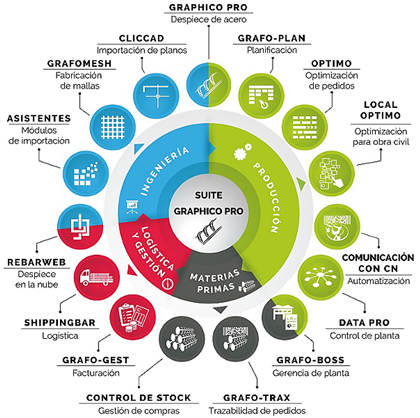
\includegraphics[scale=1]{GRAF-PRO.png}

\textbf{Personas}

La empresa cuenta con un grupo profesional de 15 personas ilusionadas en su trabajo y repartidas en áreas como desarrollo de producto, CAD, electrónica, comunicaciones, instalaciones, administración y área comercial. Además de colaboradores tecnológicos y personas altamente cualificadas en sistemas de cálculo.

La labor llevada a cabo por la empresa se realiza asimismo con el apoyo del Grupo Schnell, grupo multinacional al que pertenece, formado por 14 empresas entre productoras de maquinaria, de software y de servicios.

\item \textbf{Operación}

Planificar y controlar los procesos nos permite determinar los recursos necesarios para lograr la conformidad de los productos de software en este caso \textbf{GRAPHICO PRO} que es un software de despiece de acero con un interfaz gráfico, potente y flexible, que permite realizar despieces de elementos armados, elaborados (por posición), e incluir productos comerciales asignados a las obras.

\textbf{Características}

\begin{itemize}
\item Almacena toda la información de los proyectos, gestiona las fases de entrega y el control de los pedidos de producción.
\item Imprime informes personalizados en cada una de sus áreas: gestión de obras y clientes, pedidos de producción, etiquetas de posiciones, elementos armados y otros productos comerciales.
\item Permite duplicar información de despiece, exportar e importar niveles del proyecto, y exportar a sistemas estándares del mercado.
\item Permite a la ingeniería integrar, en un único entorno, despieces por posición o lista, esquemas de elementos armados (Cad) y definición de mallas (Grafo Mesh), además de incluir productos comerciales en cada nivel de la obra.
\item Responde a las necesidades de las grandes empresas que requieren una solución centralizada con un sistema de plantas interconectadas.
\end{itemize}

\textbf{Determinación de los requisitos}

\textbf{Requisitos funcionales}

\begin{itemize}
\item El software debe permitir el despiece de elementos estructurales armados, posiciones y productos comerciales en un mismo entorno de trabajo.
\item El software deberá pedir datos de la producción que se vaya a desarrollar.
\item El software debe soportar grande volúmenes de datos y usuarios conectados al sistema central.
\item El software debe adaptarse a los sistemas métricos internacionales.
\item El software debe conectar a entornos web para que los clientes puedan realizar seguimientos de sus pedidos.
\item El software debe contener modelos personalizados y diseños online.
\item El software debe proporcionar mensajes informativos y de error cuando existan.
\end{itemize}

\textbf{Requisitos no funcionales}

\begin{itemize}
\item Todos los procesos del software debe generar su informe correspondiente.
\item Los datos ingresados en el software deben ser estrictamente confidencial.
\item El acceso al software solo pueden ser cambiados por el administrador.
\item El software debe contar con manuales de usuarios estructurados.
\item El software debe tener una alta disponibilidad para las veces que el usuario intente acceder a el.
\item El software estará disponibles para plataformas windows 7 y 8.
\end{itemize}

\textbf{Compatibilidad de estándares del mercado}

ASTM A 615, Eurocódigo 2, BS 4449:97, EHE-08, IS 456: 2000, TS 708 -VCH, PS 90:98, DIN 488:86 NF A 35–016 :96 , ELOT 971:90, NMX-B-294-1986, JIS-G-3112, Nch-204, CIRSOC 201-2005, CBH 87 ABNT NBR 6118:2007, NSR-10, NTC 14/01/2008, NTE E.060: 2009, SABS 0100, BBK 79 (1979) SIA 162 (1989), CAN/CSA S16-01

\textbf{Diseño y desarrollo}

El software implementa las siguientes interfaces:

\begin{center}
Ventana principal
\end{center}

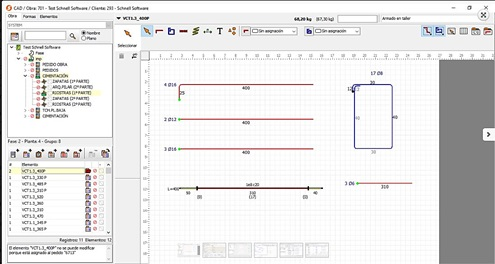
\includegraphics[scale=1]{GRAPHICO PRO 1.JPG}

\begin{center}
Datos de pedido de producción
\end{center}

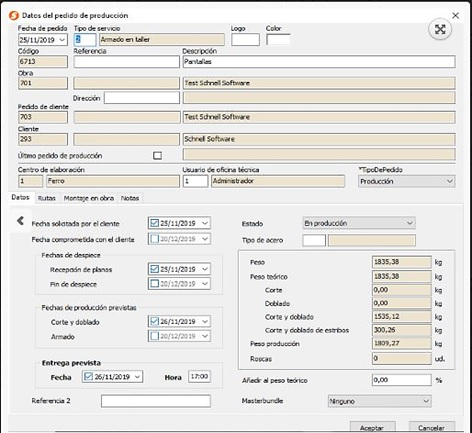
\includegraphics[scale=1]{GRAPHICO PRO 2.JPG}

\begin{center}
Trabajo en lista
\end{center}

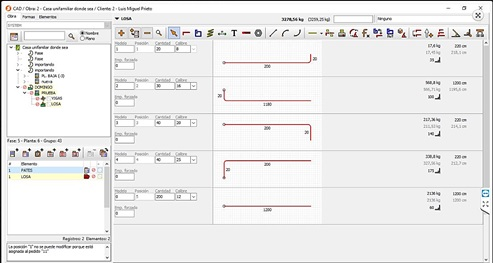
\includegraphics[scale=1]{GRAPHICO PRO - Trabajo en lista.JPG}

\begin{center}
Visor de elementos 3D
\end{center}

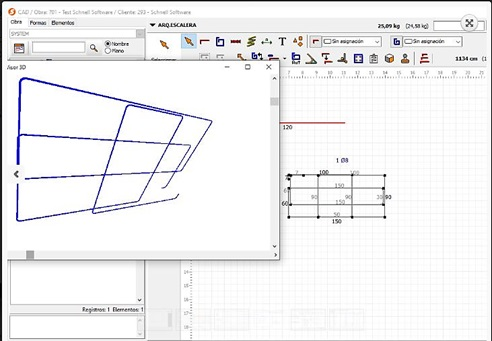
\includegraphics[scale=1]{GRAPHICO PRO - Visor de elementos 3D.JPG}

\begin{center}
Planificación de producción
\end{center}

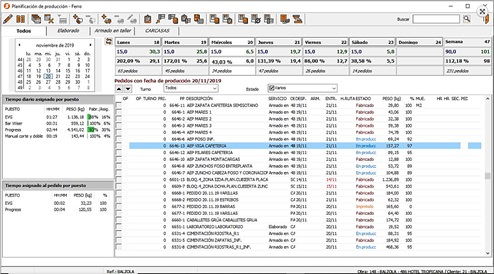
\includegraphics[scale=1]{GRAPHICO PRO - Planificacion de produccion.JPG}

\begin{center}
Gestión de pedidos de producción
\end{center}

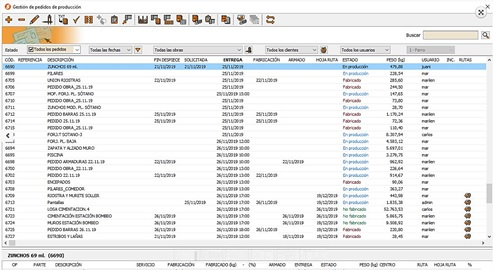
\includegraphics[scale=1]{GRAPHICO PRO - Gestion de pedidos.JPG}

\textbf{Provisión del servicio}

Graphico Pro permite asignar elementos estructurales armados completos, posiciones y productos comerciales a un pedido de producción.

El pedido de producción es la unidad de control de la planta y sobre la que se realiza toda la planificación de cargas diarias y semanales.

En todo momento el sistema le dará la información del despiece y la asignada a los pedidos de producción. El despiece se realiza en la obra y se estructura según los niveles necesarios (fase, planta, grupo). El sistema controla que una pieza asignada a un pedido no pueda enviarse de nuevo a producción. Varios pedidos de producción pueden estar asignados a un pedido comercial o del clientes.

\textbf{Alcance del control}

Asegurar que los procesos, productos y servicios suministrados externamente, no afectan de manera adversa a la capacidad de entregar productos y servicios conformes, de manera coherente, a sus clientes.

\item \textbf{Evaluación de desempeño}

Para la evaluación de desempeño se elaboró las siguientes preguntas para verificar la calidad del producto y de la empresa:

\begin{itemize}
\item ¿La empresa de servicios ha establecido, documentado e implementado un Sistema de gestión de la calidad?
\item ¿Se tienen identificados los procesos y sus interacciones?
\item ¿Se utilizan criterio y métodos que garanticen que los procesos y su control sean eficaces?
\item ¿Disponen de los recursos necesarios, así como de información que se utilice para apoyar a la operación y el seguimiento¿Se implantan las acciones necesarias para lograr resultados planificados y la mejora continua de los procesos?  de los procesos?
\item ¿Se cuenta con algún documento en que se exprese la política y los objetivos de la calidad?
\item ¿La empresa posee los procedimientos documentados requeridos para el sistema de gestión de la calidad?
\item ¿Se establece un procedimiento documentado para definir los controles necesarios para la disposición de los registros y documentos?
\item ¿Se determinan y proporcionan los recursos necesarios para mantener el sistema y mejorar su eficacia?
\item ¿El personal de la organización tiene las competencias necesarias para la prestación del servicio?
\item ¿Tiene el personal directivo las competencias necesarias para liderar?
\item ¿Se mantiene el día los registros de formación, habilidades, experiencias y competencias de los empleados?
\item ¿Están los trabajadores motivados y satisfechos con las funciones asignadas?
\item ¿Es la infraestructura de la organización adecuada para asegurar el logro de la satisfacción del cliente?
\item ¿La organización cuenta con el espacio de trabajo, los equipos y servicios de apoyo necesarios para la prestación del servicio?
\item ¿Se determina y se gestiona el ambiente de trabajo necesario para lograr la conformidad con la prestación del servicio?
\end{itemize}

SCHNELL SOFTWARE S.L. analiza y evalúa los datos y la información apropiados que surgen por el seguimiento y la
medición.

Los resultados del análisis se utilizan para evaluar:

a) La conformidad de los productos y servicios.

b) El grado de satisfacción del cliente.

c) El desempeño y la eficacia del Sistema de Gestión de Calidad.

d) Si lo planificado se ha implementado de forma eficaz.

e) La eficacia de las acciones tomadas para abordar los riesgos y oportunidades.

f) El desempeño de los proveedores externos.

g) La necesidad de mejoras en el Sistema de Gestión de Calidad.

\item \textbf{Mejoramiento}
Puntos en lo que la empresa debería mejorar.

a) Desarrollo de maquinaría con módulos de trabajo más fáciles de usar.

b) Capacitaciones de los sistemas de desarrollo.

c) Propuestas para facilitar los productos de software

d) La movilización de la maquinaria de la empresa, sus productos.

e) Detección de errores desde los requerimientos. 


\end{enumerate}
\end{document}
